\documentclass[12pt]{article}
%%%%%%%%%%%%%%%%%%%%%%%%%%%%%%%%%%%%%%%%%

\usepackage{amscd}
\usepackage{amsmath}
\usepackage{amssymb}
\usepackage{amsthm}


\usepackage{cite}

\usepackage{epsfig}
\usepackage{verbatim}
\usepackage{graphicx}
\usepackage{amsthm}
\pagestyle{empty}
\usepackage{color}




\title{\large\bf Directional Dipole Model for Subsurface Scattering}
\author{Pan An~(A0134556A)}

\begin{document}

\maketitle

\abstract{
Modern techniques for rendering different materials on computer based
systems only accounts for the interaction of light at the surface of
an object. Rendering translucent materials using Monte Carlo ray
tracing is computationally expensive due to a large number of
subsurface scattering events. Methods have been explored
to improve the efficiency for such a kind of process based on
analytical models derived from diffusion theory. These models might
improve the efficiency while leaving some redering effects missing.
The proposed approach presents an improved analytical model for
subsurface scattering  which captures translucency effects that are
present in the reference solutions but remain absent with existing
models. The proposed model(directional dipole) uses ray source diffusion instead of point
source diffusion. Directional dipole is as computationally efficient as existing models
 while it includes single scattering without relying on a separate
 Monte Carlo simulation. The result of the proposed rendering model
 is significantly closer to the references.

}





\section{Introduction}
Subsurface scattering(SSS), also known as subsurface light
transportation, is an optical physics based machanism describing the
process of light penetrating translucent materials. Different models
have been proposed in order to produce artifitial images of real life
materials. Bidirectional reflectance distribution~\cite{brdf} function was
introduced as a simple but efficient model for reflection of light at
the surface of objects. Jensen et. al.~\cite{jensen} introduced an improved model:
bidirectional subsurface scattering reflection distribution
function(BSSRDF).
The BSSRDF can describe light transport between any two rays that hit a surface, whereas the BRDF assumes that light entering a material leaves the material at the same position
BSSRDF can be described as following:

$$
S(x_i, \vec{\omega_i}; x_o, \vec{\omega_o})  = S_d(x_i,
\vec{\omega_i}; x_o, \vec{\omega_o}) +S^{(1)}(x_i, \vec{\omega_i};
x_o, \vec{\omega_o})
$$

where $S$ is the bidirectional subsurface scattering reflection distribution
function. $S_d$ and $S^{(1)}$ are the diffusion approximation and
single scattering term.

The result of the rendering with BSSRDF would depend on the physical
characteristics such as absorption coefficient, index of retraction,
scattering coefficient, etc. A list of such parameters has been
measured in Jensen's work. Gkioulekas et. al.~\cite{materials} studied on the
physical characteristics of daily materials. Gkioulekas et. al. used a
series of techniques and algorithms in order to achieve a set of data
for daily materials such as wine, milk, coffee etc. Based on their
analysis we are able to achieve a better result in multimedia
rendering.

\section{proposal}
Directional dipole~\cite{direction} method is proposed to improve the efficiency and
accuracy of translucent material rendering process.
The dipole approximation for subsurface scattering has proven to be a
fast practical way of rendering such materials. This standard dipole
model is however built upon a number of assumptions which are often
violated. One significant assumption is that incident light is
directionally uniform. However, in real physical world, this
assumption is rarely satisfied.

The standard dipole model should be integrated along the refracted
ray.
A standard dipole model uses two point sources to handle boundary
conditions. The points are displaced along the normal at the point of
incidence. Our model uses two directional sources that are displaced
along the normal of a plane containing the points of incidence and
emergence. It calculates the approximation of the multipole by capturing scattering due to a
normally incident light ray. This displacement
of the real source leads to a modified distance to the real source
based on the assumption that the ray is normally incident on a planar surface.

Directional dipole method increases the rendering efficiency by
conducting precomputation on the light source instead of displacing
the real source.

\begin{figure}[!ht]
  \centering
  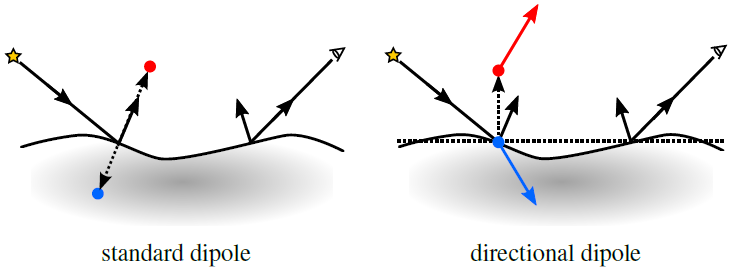
\includegraphics[scale=0.5]{dipoles.png}
  \caption{Standard dipole method(left) and directional dipole.}
  \label{fig:dipole}
\end{figure}

The proposed method  focuses in this paper is to find an improved
analytical model for subsurface scattering. 
The diffusive part of the
proposed BSSRDF is as following:


$$
S_d({\bf x}_i, \vec{\omega_i}; {\bf x}_o)  = S'_d({\bf x}_0 - {\bf x}_i,
\vec{\omega_{12}}, d_r) - S'_d({\bf x}_0 - {\bf x}_v, \vec{\omega_v}
d_r)
$$
Details of the explaination will be given at the second
presentation. \ref{fig:directional} explains the dipole configurations of
the proposed method. Similar to dipole with point sources, directional
dipole uses ray sources.We mirror the direction of the refracted
ray(blue) $\vec{\omega_{12}}$ in a modified tangent
plane to find the direction $\vec{\omega_v}$ of the virtual source.
The origin of the virtual source is displaced along the normal of this modified plane.

\begin{figure}[!ht]
  \centering
  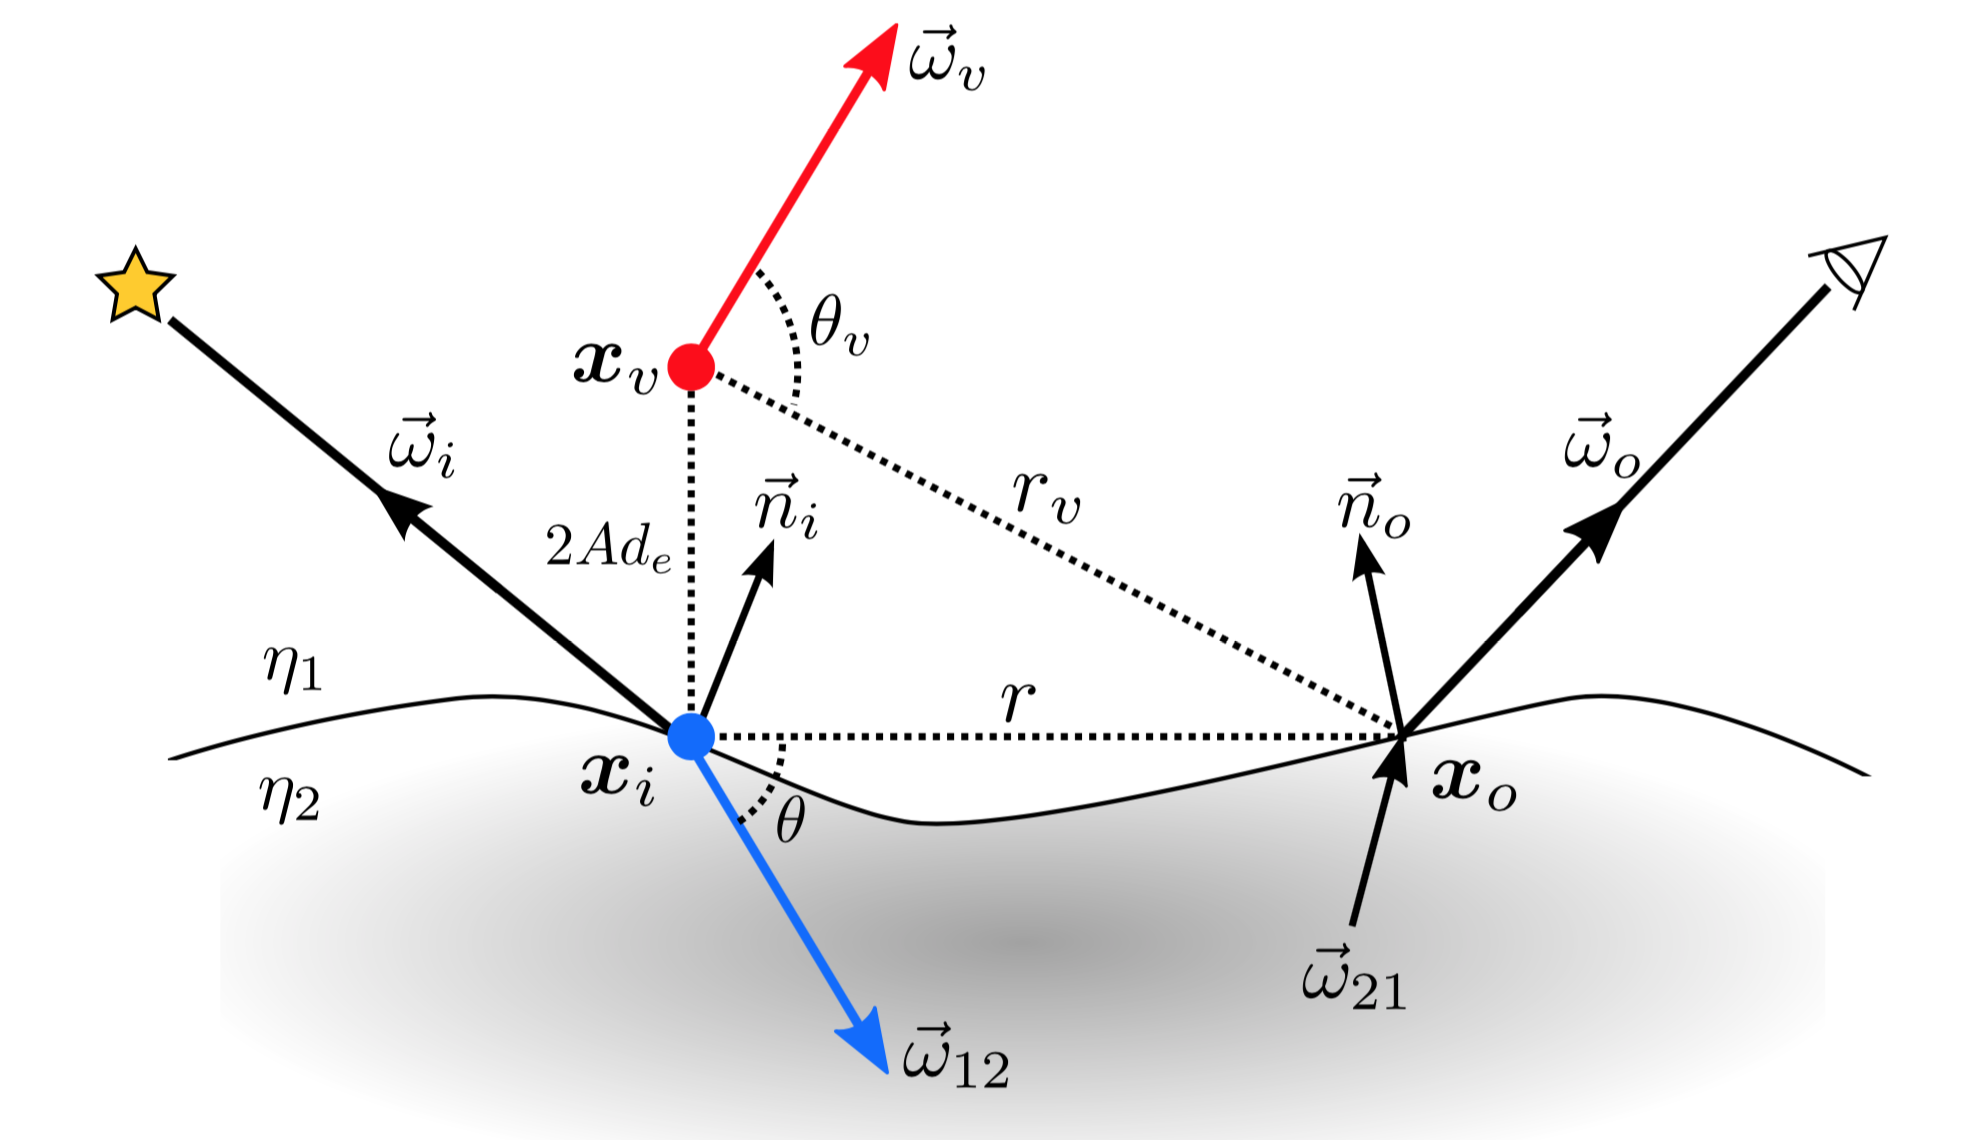
\includegraphics[scale=0.2]{direct.png}
  \caption{Directional Dipole}
  \label{fig:directional}
\end{figure}

The implementation of directional dipole contains monte carlo
integration, as well as Jensen's work. Directional dipole  integrates
the BSSRDF in a progressive path tracer by distributing points evenly
across the surface of the translucent object using a dart throwing
technique. A new set of points is sampled iteratively, and, for every
sampled surface point, the incident illumination is sampled from one
direction. Photon mapping can also be done with other algorithms
like k-nearest neighbor orkd-trees, as was also mentioned by Jensen.

For hierarchical integration,
  a simpler approach of utilizing the existing
implementation of the hierarchical integration method is used.


\bibliography{papers}{}

\bibliographystyle{plain}





\end{document}

%%% Local Variables:
%%% mode: latex
%%% TeX-master: t
%%% End:
